\mfpicnumber{1}

\opengraphsfile{GraphsofEquations}

\setcounter{footnote}{0}

\label{GraphsofEquations}

In the previous section, we said that one could describe relations algebraically using equations.  In this section, we begin to explore this topic in greater detail.  The main idea of this section is

\medskip

\colorbox{ResultColor}{\bbm

\smallskip

\centerline{\textbf{The Fundamental Graphing Principle}}

\label{fgp} \index{equation ! graph of} \index{graph ! of an equation} \index{Fundamental Graphing Principle ! for equations} \index{relation ! Fundamental Graphing Principle}

The graph of an equation is the set of points which satisfy the equation.  That is, a point $(x,y)$ is on the graph of an equation if and only if $x$ and $y$ satisfy the equation.

\smallskip

\ebm}

\medskip

\begin{ex} Determine if $(2,-1)$ is on the graph of $x^2 + y^3 = 1$.

\medskip

{\bf Solution.}  To check, we substitute $x=2$ and $y=-1$ into the equation and see if the equation is satisfied

\setlength{\extrarowheight}{2pt}

\[ \begin{array}{rclr}   
 (2)^2+(-1)^3 & \stackrel{?}{=} & 1 & \\ 
            3 & \neq & 1 & \\ 
            \end{array} \]

Hence, $(2,-1)$ is \textbf{not} on the graph of $x^2 + y^3 = 1$.

\qed

\end{ex}

We could spend hours randomly guessing and checking to see if points are on the graph of the equation.  A more systematic approach is outlined in the following example.

\begin{ex}  Graph $x^2 + y^3 = 1$.

\label{firstequgraph}

\medskip

{\bf Solution.}  To  efficiently generate points on the graph of this equation, we first solve for $y$

\[ \begin{array}{rclr} 
    x^2 + y^3 & = & 1 & \\ 
          y^3 & = & 1 - x^2 & \\
\sqrt[3]{y^3} & = & \sqrt[3]{1 - x^2} & \\
            y & = & \sqrt[3]{1 - x^2} & \\ 
            \end{array} \]

We now substitute a value in for $x$, determine the corresponding value $y$, and plot the resulting point, $(x,y)$.  For example, for $x=-3$, we substitute

\[y = \sqrt[3]{1 - x^2} = \sqrt[3]{1 - (-3)^2} = \sqrt[3]{-8} = - 2,\]

so the point $(-3, -2)$ is on the graph.  Continuing in this manner, we generate a table of points which are on the graph of the equation.  These points are then plotted in the plane as shown below.

\hspace{.75in} \begin{tabular}{m{2.25in}m{3in}}

$\begin{array}{|r||c|c|}  \hline

  x & y & (x,y) \\ \hline
 -3 & -2 & (-3, -2) \\  \hline
 -2 & -\sqrt[3]{3}& (-2,-\sqrt[3]{3}) \\  \hline
 -1 & 0 & ( -1, 0) \\  \hline
  0 & 1& ( 0 , 1) \\  \hline
  1 & 0 & ( 1, 0) \\  \hline
  2 & -\sqrt[3]{3}& (2,-\sqrt[3]{3}) \\  \hline
  3 & -2 & (3, -2) \\  \hline

\end{array}$ & 

\begin{mfpic}[20]{-5}{5}{-4}{4}
\point[4pt]{(-3,-2),(-2,-1.4422), (-1,0), (0,1), (3,-2),(2,-1.4422), (1,0)}
\axes
\xmarks{-4,-3,-2,-1,1,2,3,4}
\ymarks{-3,-2,-1,1,2,3}
\tlabel[cc](5,-0.5){$x$}
\tlabel[cc](0.5,4){$y$}
\tlpointsep{5pt}
\scriptsize
\axislabels {x}{{$-4 \hspace{7pt}$} -4, {$-3 \hspace{7pt}$} -3, {$-2 \hspace{7pt}$} -2, {$-1 \hspace{7pt}$} -1, {$1$} 1, {$2$} 2, {$3$} 3, {$4$} 4}
\axislabels {y}{{$-3$} -3, {$-2$} -2, {$-1$} -1, {$1$} 1, {$2$} 2, {$3$} 3}
\normalsize
\end{mfpic} \\

\end{tabular}

Remember, these points constitute only a small \textbf{sampling} of the points on the graph of this equation.  To get a better idea of the shape of the graph, we could plot more points until we feel comfortable `connecting the dots.'  Doing so would result in a curve similar to the one pictured below on the far left.

\medskip

\begin{tabular}{m{2.1in}m{2in}m{2in}}
\begin{mfpic}[15]{-5}{5}{-4}{4}
\arrow \reverse \parafcn{-2.5,1,0.1}{(sqrt(1-t^3),t)}
\arrow \reverse \parafcn{-2.5,1,0.1}{(-1*sqrt(1-t^3),t)}
\point[3pt]{(-3,-2),(-2,-1.4422), (-1,0), (0,1), (3,-2),(2,-1.4422), (1,0)}
\axes
\tlabel[cc](5,-0.5){$x$}
\tlabel[cc](0.5,4){$y$}
\xmarks{-4,-3,-2,-1,1,2,3,4}
\ymarks{-3,-2,-1,1,2,3}
\tlpointsep{5pt}
\scriptsize
\axislabels {x}{{$-4 \hspace{7pt}$} -4, {$-3 \hspace{7pt}$} -3, {$-2 \hspace{7pt}$} -2, {$-1 \hspace{7pt}$} -1, {$1$} 1, {$2$} 2, {$3$} 3, {$4$} 4}
\axislabels {y}{{$-3$} -3, {$-2$} -2, {$-1$} -1, {$1$} 1, {$2$} 2, {$3$} 3}
\end{mfpic} & 

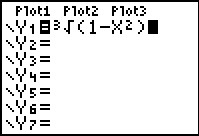
\includegraphics[width=1.9in]{./RelationsandFunctionsGraphics/Equation01.jpg} & 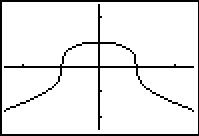
\includegraphics[width=1.9in]{./RelationsandFunctionsGraphics/Equation02.jpg} \\

\end{tabular}

Don't worry if you don't get all of the little bends and curves just right $-$ Calculus is where the art of precise graphing takes center stage.  For now, we will settle with our naive `plug and plot' approach to graphing.  If you feel like all of this tedious computation and plotting is beneath you, then you can reach for a graphing calculator, input the formula as shown above, and graph.

\qed

\end{ex}

\medskip

Of all of the points on the graph of an equation, the places where the graph crosses the axes hold special significance.  These are called the \textbf{intercepts} \index{intercept ! definition of} of the graph.  Intercepts come in two distinct varieties: $x$-intercepts and $y$-intercepts.  They are defined below.

\medskip

\colorbox{ResultColor}{\bbm

\smallskip

\begin{defn}  Suppose the graph of an equation is given.

\label{interceptsdefn}

\begin{itemize}

\item  A point at which a graph meets the $x$-axis is called an \index{$x$-intercept} \textbf{\boldmath $x$-intercept} of the graph.

\item  A point at which a graph meets the $y$-axis is called an \index{$y$-intercept} \textbf{\boldmath $y$-intercept} of the graph.

\smallskip

\end{itemize}

\end{defn}

\ebm}

\medskip

In our previous example the graph had two $x$-intercepts, $(-1,0)$ and $(1,0)$, and one $y$-intercept, $(0,1)$.  The graph of an equation can have any number of intercepts, including none at all!  Since $x$-intercepts lie on the $x$-axis, we can find them by setting $y = 0$ in the equation.  Similarly, since $y$-intercepts lie on the $y$-axis, we can find them by setting $x = 0$ in the equation.  Keep in mind, intercepts are \emph{points} and therefore must be written as ordered pairs.  To summarize,

\medskip

\colorbox{ResultColor}{\bbm

\smallskip

\centerline{\textbf{Steps for Finding the Intercepts of the Graph of an Equation}}

\medskip

\hspace{.17in} Given an equation involving $x$ and $y$: \index{intercept ! location of}

\begin{itemize}

\item the $x$-intercepts always have the form $(x,0)$;  to find the $x$-intercepts of the graph, set $y=0$ and solve for $x$.  

\item   $y$-intercepts always have the form $(0,y)$; to find the $y$-intercepts of the graph, set $x=0$ and solve for $y$. 

\smallskip

\end{itemize}

\ebm}

\medskip

Another fact which you may have noticed about the graph in the previous example is that it seems to be symmetric about the $y$-axis.  To actually prove this analytically, we assume $(x,y)$ is a generic point on the graph of the equation. That is, we assume  $x^2 + y^3 = 1$.  As we learned in Section \ref{CartesianPlane},  the point symmetric to $(x,y)$ about the $y$-axis is $(-x,y)$.  To show the graph is symmetric about the $y$-axis, we need to show that $(-x,y)$ is on the graph whenever $(x,y)$ is.  In other words, we need to show $(-x,y)$ satisfies the equation $x^2 + y^3 = 1$ whenever $(x,y)$ does.  Substituting gives

\setlength{\extrarowheight}{2pt}

\[ \begin{array}{rclr}   
(-x)^2+(y)^3 & \stackrel{?}{=} & 1 & \\
   x^2 + y^3 & \stackrel{\checkmark}{=} & 1 & \\ 
   \end{array} \]

When we substituted $(-x,y)$ into the equation $x^2 + y^3 = 1$, we obtained the original equation back when we simplified.  This means $(-x, y)$ satisfies the equation and hence is on the graph.  In this way, we can check whether the graph of a given equation possesses any of the symmetries discussed in Section \ref{CartesianPlane}.  The results are summarized below.

\medskip

\colorbox{ResultColor}{\bbm

\smallskip

\centerline{\textbf{Steps for Testing if the Graph of an Equation Possesses Symmetry}}
\phantomsection
\label{symmetrytestequations}

\medskip

\hspace{.17in} To test the graph of an equation for symmetry \index{symmetry ! testing an equation for} 

\begin{itemize}

\item About the $y$-axis: Substitute $(-x,y)$ into the equation and simplify.  If the result is equivalent to the original equation, the graph is symmetric about the $y$-axis.

\item About the $x$-axis: Substitute $(x,-y)$ into the equation and simplify.  If the result is equivalent to the original equation, the graph is symmetric about the $x$-axis.

\item About the origin: Substitute $(-x,-y)$ into the equation and simplify. If the result is equivalent to the original equation, the graph is symmetric about the origin.

\smallskip

\end{itemize}

\ebm}

\medskip

Intercepts and symmetry are two tools which can help us sketch the graph of an equation analytically, as evidenced in the next example.

\begin{ex}  Find the $x$- and $y$-intercepts (if any) of the graph of $(x-2)^2 + y^2 = 1$. Test for symmetry.  Plot additional points as needed to complete the graph.
\label{secondequgraph}

\medskip

{\bf Solution.} To look for $x$-intercepts, we set $y=0$ and solve:

\[ \begin{array}{rclr}   

(x-2)^2 + y^2 & = & 1 & \\ 
(x-2)^2 + 0^2 & = & 1 & \\ 
(x-2)^2 & = & 1 & \\
\sqrt{(x-2)^2} & = & \sqrt{1} & \mbox{extract square roots}\\
x - 2 & = & \pm 1 & \\
x  & = & 2 \pm 1 & \\
x  & = & 3, 1 & \\

\end{array} \]

We get \textbf{two} answers for $x$ which correspond to \textbf{two} $x$-intercepts:  $(1,0)$ and $(3,0)$.    Turning our attention to $y$-intercepts, we set $x=0$ and solve:

\[ \begin{array}{rclr}   

(x-2)^2 + y^2 & = & 1 & \\ 
(0-2)^2 + y^2 & = & 1 & \\ 
4 + y^2 & = & 1 & \\
y^2 & = & -3 & \\

\end{array} \]

Since there is no real number which squares to a negative number (Do you remember why?), we are forced to conclude that the graph has \textbf{no} $y$-intercepts.

\medskip

Plotting the data we have so far, we get

\begin{center}

\begin{mfpic}[15]{-1}{5}{-3}{3}
\point[3pt]{(1,0), (3,0)}
\footnotesize
\tlabel[cc](1,0.5){$(1,0)$}
\tlabel[cc](3,0.5){$(3,0)$}
\normalsize
\axes
\tlabel[cc](5,-0.5){$x$}
\tlabel[cc](0.5,3){$y$}
\xmarks{1,2,3,4}
\ymarks{-2,-1,1,2}
\tlpointsep{5pt}
\scriptsize
\axislabels {x}{{$1$} 1, {$2$} 2, {$3$} 3, {$4$} 4}
\axislabels {y}{{$-2$} -2, {$-1$} -1, {$1$} 1, {$2$} 2}
\normalsize
\end{mfpic}

\end{center}

Moving along to symmetry, we can immediately dismiss the possibility that the graph is symmetric about the $y$-axis or the origin.  If the graph possessed either of these symmetries, then the fact that $(1,0)$ is on the graph would mean $(-1,0)$ would have to be on the graph. (Why?)  Since $(-1,0)$ would be another $x$-intercept (and we've found all of these), the graph can't have $y$-axis or origin symmetry.  The only symmetry left to test is symmetry about the $x$-axis.   To that end, we substitute $(x,-y)$ into the equation and simplify

\[ \begin{array}{rclr}   

(x-2)^2 + y^2 & = & 1 & \\ 
(x-2)^2 + (-y)^2 & \stackrel{?}{=} & 1 & \\ 
(x-2)^2 + y^2 & \stackrel{\checkmark}{=} & 1 & \\

\end{array} \]

Since we have obtained our original equation, we know the graph is symmetric about the $x$-axis.  This means we can cut our `plug and plot' time in half:  whatever happens below the $x$-axis is reflected above the $x$-axis, and vice-versa.  Proceeding as we did in the previous example, we obtain

\begin{center}

\begin{mfpic}[15]{-1}{5}{-3}{3}
\point[3pt]{(1,0), (3,0)}
\circle{(2,0),1}
\axes
\tlabel[cc](5,-0.5){$x$}
\tlabel[cc](0.5,3){$y$}
\xmarks{1,2,3,4}
\ymarks{-2,-1,1,2}
\tlpointsep{5pt}
\scriptsize
\axislabels {x}{{$1$} 1, {$2$} 2, {$3$} 3, {$4$} 4}
\axislabels {y}{{$-2$} -2, {$-1$} -1, {$1$} 1, {$2$} 2}
\normalsize
\end{mfpic}

\end{center}

\qed

\end{ex}

A couple of remarks are in order.  First, it is entirely possible to choose a value for $x$ which does not correspond to a point on the graph.  For example, in the previous example, if we solve for $y$ as is our custom, we get:
\[y = \pm \sqrt{1-(x-2)^2}.\]
Upon substituting $x=0$ into the equation, we would obtain
\[y = \pm \sqrt{1 - (0-2)^2} = \pm \sqrt{1 - 4} = \pm \sqrt{-3},\]
which is not a real number.  This means there are no points on the graph with an $x$-coordinate of $0$.  When this happens, we move on and try another point.  This is another drawback of the `plug-and-plot' approach to graphing equations.  Luckily, we will devote much of the remainder of this book developing techniques which allow us to graph entire families of equations quickly.\footnote{Without the use of a calculator, if you can believe it!}  Second, it is instructive to show what would have happened had we tested the equation in the last example for symmetry about the $y$-axis.  Substituting $(-x,y)$ into the equation yields

\[ \begin{array}{rclr}  

(x-2)^2 + y^2 & = & 1 & \\
(-x-2)^2 + y^2 & \stackrel{?}{=} & 1 & \\
((-1)(x+2))^2 + y^2 & \stackrel{?}{=} & 1 & \\
(x+2)^2 + y^2 & \stackrel{?}{=} & 1. & \\

\end{array} \]

This last equation does not \textbf{appear} to be equivalent to our original equation.  However, to \textbf{prove} it is not symmetric about the $y$-axis, we need to find a point $(x,y)$ on the graph whose reflection $(-x,y)$ is not. Our $x$-intercept $(1,0)$ fits this bill nicely, since if we substitute $(-1,0)$ into the equation we get

\[ \begin{array}{rclr}   

(x-2)^2+y^2 & \stackrel{?}{=} & 1 & \\
(-1-2)^2 + 0^2 & \neq & 1 & \\
9 & \neq & 1. & 

\end{array} \]

This proves that $(-1,0)$ is not on the graph.

\newpage

\subsection{Exercises}

\begin{enumerate}

\item For each equation given below

\begin{itemize}

\item Find the $x$- and $y$-intercept(s) of the graph, if any exist.

\item Following the procedure in Example \hspace{-.1in} ~\ref{firstequgraph}, create a table of sample points on the graph of the equation.

\item Plot the sample points and create a rough sketch of the graph of the equation.

\item Test for symmetry.  If the equation appears to fail any of the symmetry tests, find a point on the graph of the equation whose reflection fails to be on the graph as was done at the end of Example \hspace{-.1in} ~\ref{secondequgraph}

\end{itemize}

\begin{multicols}{2}

\begin{enumerate}

\item $y = x^{2} + 1$
\item  $y = x^2-2x-8$

\item $y = x^{3} - x$
\item  $y = \frac{x^3}{4} - 3x$


\item $y = \sqrt{x - 2}$
\item  $y = 2 \sqrt{x+4} - 2$

\item $3x - y = 7$
\item  $3x-2y = 10$

\item  $(x+2)^2+y^2 = 16$

\item $x^{2} - y^{2} = 1$
\item  $4y^2 - 9x^2 = 36$


\item $x^{3}y = -4$ 

\end{enumerate}

\end{multicols}

\item The procedures which we have outlined in the Examples of this section and used in the exercises given above all rely on the fact that the equations were ``well-behaved''.  Not everything in Mathematics is quite so tame, as the following equations will show you.  Discuss with your classmates how you might approach graphing these equations.  What difficulties arise when trying to apply the various tests and procedures given in this section?  For more information, including pictures of the curves, each curve name is a link to its page at www.wikipedia.org.  For a much longer list of fascinating curves, click \href{http://en.wikipedia.org/wiki/List_of_curves}{\underline{here}}.
\label{listofcurves}

\begin{multicols}{2}

\begin{enumerate}

\item $x^{3} + y^{3} - 3xy = 0\;$ \href{http://en.wikipedia.org/wiki/Folium_of_descartes}{\underline{Folium of Descartes}}
\item $x^{4} = x^{2} + y^{2}\;$ \href{http://en.wikipedia.org/wiki/Kampyle_of_Eudoxus}{\underline{Kampyle of Eudoxus}}
\item $y^{2} = x^{3} + 3x^{2}\;$ \href{http://en.wikipedia.org/wiki/Tschirnhausen_cubic}{\underline{Tschirnhausen cubic}}
\item $(x^{2} + y^{2})^{2} = x^{3} + y^{3}\;$ \href{http://en.wikipedia.org/wiki/Crooked_egg_curve}{\underline{Crooked egg}} 

\end{enumerate}

\end{multicols}

\end{enumerate}

\newpage

\subsection{Answers}

\begin{enumerate}

\item \begin{multicols}{2} \raggedcolumns

\begin{enumerate}

\item $y = x^{2} + 1$

\begin{flushleft}

The graph has no $x$-intercepts \smallskip

$y$-intercept: $(0, 1)$  \smallskip

$\begin{array}{|r||c|c|}  

\hline
 x & y & (x,y) \\ \hline
-2 & 5 & (-2, 5) \\  \hline
-1 & 2 & (-1, 2) \\ \hline
 0 & 1 & (0, 1) \\ \hline
 1 & 2 & (1, 2) \\ \hline
 2 & 5 & (2, 5) \\ \hline
 
\end{array} $ \smallskip

\begin{mfpic}[10]{-3}{3}{-1}{6}
\point[3pt]{(-2,5), (-1,2), (0,1), (1,2), (2,5)}
\axes
\tlabel[cc](3,-0.5){\scriptsize $x$}
\tlabel[cc](0.5,6){\scriptsize $y$}
\xmarks{-2,-1,1,2}
\ymarks{1,2,3,4,5}
\tlpointsep{4pt}
\axislabels {x}{{\tiny $-2 \hspace{6pt}$} -2, {\tiny $-1 \hspace{6pt}$} -1, {\tiny $1$} 1, {\tiny $2$} 2}
\axislabels {y}{{\tiny $1$} 1, {\tiny $2$} 2, {\tiny $3$} 3, {\tiny $4$} 4, {\tiny $5$} 5}
\arrow \reverse \arrow \function{-2.3, 2.3, 0.1}{x**2+1}
\end{mfpic}

\smallskip

The graph is not symmetric about the $x$-axis (e.g. $(2, 5)$ is on the graph but $(2, -5)$ is not) \smallskip

The graph is symmetric about the $y$-axis \smallskip

The graph is not symmetric about the origin (e.g. $(2, 5)$ is on the graph but $(-2, -5)$ is not)

\end{flushleft}

\vspace{4in}

\item $y = x^{2} -2x-8$

\begin{flushleft}

$x$-intercepts:  $(4,0)$, $(-2,0)$ \smallskip

$y$-intercept: $(0, -8)$  \smallskip

$\begin{array}{|r||c|c|}  

\hline
 x & y & (x,y) \\ \hline
-3 & 7 & (-3,7) \\ \hline
-2 & 0 & (-2, 0) \\  \hline
-1 & -5 & (-1, -5) \\ \hline
 0 & -8 & (0, -8) \\ \hline
 1 & -9 & (1, -9) \\ \hline
 2 & -8 & (2, -8) \\ \hline
 3 & -5 & (3,-5) \\ \hline
 4 & 0 & (4,0) \\ \hline
 5 & 7 & (5,7) \\ \hline
 
\end{array}$  \smallskip

\begin{mfpic}[7]{-4}{6}{-10}{8}
\point[3pt]{(-3,7), (-2,0), (-1,-5), (0,-8), (1,-9), (2,-8), (3,-5), (4,0), (5,7)}
\axes
\tlabel[cc](6,-0.5){\scriptsize $x$}
\tlabel[cc](0.5,8){\scriptsize $y$}
\xmarks{-3,-2,-1,1,2,3,4,5}
\ymarks{-9,-8,-7,-6,-5,-4,-3,-2,-1,1,2,3,4,5,6,7}
\tlpointsep{4pt}
\axislabels {x}{{\tiny $-3 \hspace{6pt}$} -3,{\tiny $-2 \hspace{6pt}$} -2, {\tiny $-1 \hspace{6pt}$} -1, {\tiny $1$} 1, {\tiny $2$} 2, {\tiny $3$} 3, {\tiny $4$} 4, {\tiny $5$} 5}
\axislabels {y}{{\tiny $-9$} -9, {\tiny $-8$} -8, {\tiny $-7$} -7, {\tiny $-6$} -6, {\tiny $-5$} -5, {\tiny $-4$} -4, {\tiny $-3$} -3, {\tiny $-2$} -2, {\tiny $1$} 1, {\tiny $2$} 2, {\tiny $3$} 3, {\tiny $4$} 4, {\tiny $5$} 5, {\tiny $6$} 6, {\tiny $7$} 7}
\arrow \reverse \arrow \function{-3.1, 5.1, 0.1}{x**2-2*x-8}
\end{mfpic}

\smallskip

The graph is not symmetric about the $x$-axis (e.g. $(-3, 7)$ is on the graph but $(-3, -7)$ is not) \smallskip

The graph is  not symmetric about the $y$-axis (e.g. $(-3, 7)$ is on the graph but $(3, 7)$ is not) \smallskip

The graph is not symmetric about the origin (e.g. $(-3, 7)$ is on the graph but $(3, -7)$ is not)

\end{flushleft}

\pagebreak

\item $y = x^{3} - x$

\begin{flushleft}

$x$-intercepts: $(-1, 0), (0, 0), (1, 0)$ \smallskip

$y$-intercept: $(0, 0)$ \smallskip

$\begin{array}{|r||c|c|}  

\hline
 x &  y & (x,y) \\ \hline
-2 & -6 & (-2, -6) \\  \hline
-1 &  0 & (-1, 0) \\ \hline
 0 &  0 & (0, 0) \\ \hline
 1 &  0 & (1, 0) \\ \hline
 2 &  6 & (2, 6) \\ \hline
 
\end{array} $ \smallskip

\begin{mfpic}[10]{-3}{3}{-7}{7}
\point[3pt]{(-2,-6), (-1,0), (0,0), (1,0), (2,6)}
\axes
\tlabel[cc](3,-0.5){\scriptsize $x$}
\tlabel[cc](0.5,7){\scriptsize $y$}
\xmarks{-2,-1,1,2}
\ymarks{-6,-5,-4,-3,-2,-1,1,2,3,4,5,6}
\tlpointsep{4pt}
\axislabels {x}{{\tiny $-2 \hspace{6pt}$} -2, {\tiny $-1 \hspace{6pt}$} -1, {\tiny $1$} 1, {\tiny $2$} 2}
\axislabels {y}{{\tiny $-6$} -6,{\tiny $-5$} -5,{\tiny $-4$} -4,{\tiny $-3$} -3,{\tiny $-2$} -2,{\tiny $-1$} -1, {\tiny $1$} 1, {\tiny $2$} 2, {\tiny $3$} 3, {\tiny $4$} 4, {\tiny $5$} 5, {\tiny $6$} 6}
\arrow \reverse \arrow \function{-2.1, 2.1, 0.1}{x**3-x}
\end{mfpic}

\smallskip

The graph is not symmetric about the $x$-axis. (e.g. $(2, 6)$ is on the graph but $(2, -6)$ is not) \smallskip

The graph is not symmetric about the $y$-axis. (e.g. $(2, 6)$ is on the graph but $(-2, 6)$ is not) \smallskip

The graph is symmetric about the origin.

\end{flushleft}

\vspace{2in}

\item $y = \frac{x^3}{4} - 3x$

\begin{flushleft}

$x$-intercepts: $\left(\pm 2\sqrt{3}, 0\right)$   \smallskip

$y$-intercept: $(0,0)$ \smallskip

$\begin{array}{|r||c|c|}  

\hline
 x & y & (x,y) \\ \hline
 -4 & -4 & (-4, -4) \\  \hline
 -3 & \frac{9}{4} & \left(-3, \frac{9}{4} \right) \\ \hline
 -2 & 4 & (-2, 4) \\ \hline
-1 & \frac{11}{4} & \left(-1, \frac{11}{4}\right) \\ \hline
 0 & 0 & (0,0) \\ \hline
 1 & -\frac{11}{4} & \left(1, -\frac{11}{4}\right) \\ \hline
 2 & -4 & (2, -4) \\ \hline
 3 & -\frac{9}{4} & \left(3, -\frac{9}{4} \right) \\ \hline
 4 & 4 & (4, 4) \\  \hline
 
\end{array} $ \smallskip

\begin{mfpic}[10]{-5}{5}{-5}{5}

\point[3pt]{(-4,-4), (-3.4641, 0), (-3, 2.25), (-2,4), (-1,2.75), (0,0), (4,4), (3.4641, 0),(3, -2.25), (2,-4), (1,-2.75)}

\axes

\tlabel[cc](5,-0.5){\scriptsize $x$}

\tlabel[cc](0.5,5){\scriptsize $y$}

\xmarks{-4,-3,-2,-1,1,2,3,4}

\ymarks{-4,-3,-2,-1,1,2,3,4}

\tlpointsep{4pt}

\axislabels {x}{{\tiny $-4 \hspace{6pt}$} -4,{\tiny $-3 \hspace{6pt}$} -3,{\tiny $-2 \hspace{6pt}$} -2,{\tiny $-1 \hspace{6pt}$} -1,{\tiny $1$} 1, {\tiny $2$} 2, {\tiny $3$} 3, {\tiny $4$} 4}

\axislabels {y}{{\tiny $-1$} -1, {\tiny $-2$} -2, {\tiny $-3$} -3, {\tiny $-4$} -4,{\tiny $1$} 1, {\tiny $2$} 2, {\tiny $3$} 3, {\tiny $4$} 4}

\arrow \reverse \arrow \function{-4.1, 4.1, 0.1}{0.25*(x**3)-3*x}

\end{mfpic}

\smallskip

The graph is not symmetric about the $x$-axis (e.g. $(-4, -4)$ is on the graph but $(-4, 4)$ is not) \smallskip

The graph is not symmetric about the $y$-axis (e.g. $(-4, -4)$ is on the graph but $(4, -4)$ is not) \smallskip

The graph is symmetric about the origin

\end{flushleft}

\pagebreak


\item $y = \sqrt{x - 2}$

\begin{flushleft}

$x$-intercept: $(2, 0)$  \smallskip

The graph has no $y$-intercepts \smallskip

$\begin{array}{|r||c|c|}  

\hline
 x & y & (x,y) \\ \hline
 2 & 0 & (2, 0) \\  \hline
 3 & 1 & (3, 1) \\ \hline
 6 & 2 & (6, 2) \\ \hline
11 & 3 & (11, 3) \\ \hline
 
\end{array} $ \smallskip

\begin{mfpic}[10]{-1}{12}{-1}{4}

\point[3pt]{(2,0), (3,1), (6,2), (11,3)}

\axes

\tlabel[cc](12,-0.5){\scriptsize $x$}

\tlabel[cc](0.5,4){\scriptsize $y$}

\xmarks{1,2,3,4,5,6,7,8,9,10,11}

\ymarks{1,2,3}

\tlpointsep{4pt}

\axislabels {x}{{\tiny $1$} 1, {\tiny $2$} 2, {\tiny $3$} 3, {\tiny $4$} 4, {\tiny $5$} 5, {\tiny $6$} 6, {\tiny $7$} 7, {\tiny $8$} 8, {\tiny $9$} 9, {\tiny $10$} 10, {\tiny $11$} 11}

\axislabels {y}{{\tiny $1$} 1, {\tiny $2$} 2, {\tiny $3$} 3}

\arrow \function{2, 12, 0.1}{sqrt(x - 2)}

\end{mfpic}

\smallskip

The graph is not symmetric about the $x$-axis (e.g. $(3, 1)$ is on the graph but $(3, -1)$ is not) \smallskip

The graph is not symmetric about the $y$-axis (e.g. $(3, 1)$ is on the graph but $(-3, 1)$ is not) \smallskip

The graph is not symmetric about the origin (e.g. $(3, 1)$ is on the graph but $(-3, -1)$ is not)

\end{flushleft}

\vspace{4in}

\item $y = 2 \sqrt{x+4} - 2$

\begin{flushleft}

$x$-intercept: $(-3,0)$  \smallskip

$y$-intercept: $(0,2)$ \smallskip

$\begin{array}{|r||c|c|}  

\hline
 x &  y & (x,y) \\ \hline
-4 & -2 & (-4, -2) \\ \hline
-3 & 0 & (-3,0 ) \\  \hline
-2 & 2 \sqrt{2} -2 & \left(-2, \sqrt{2} -2 \right) \\ \hline
 -1 & 2 \sqrt{3} -2 & \left(-2, \sqrt{3} -2 \right) \\ \hline
 0 & 2 & (0, 2) \\ \hline
 1 & 2 \sqrt{5} -2 & \left(-2, \sqrt{5} -2 \right) \\ \hline
 
\end{array} $ \smallskip

\begin{mfpic}[10]{-5}{3}{-4}{4}

\point[3pt]{(-4,-2), (-3,0), (-2, 0.8284), (-1, 1.464), (0,2), (1,2.472)}

\axes

\tlabel[cc](3,-0.5){\scriptsize $x$}

\tlabel[cc](0.5,4){\scriptsize $y$}

\xmarks{-4,-3,-2,-1,1,2}

\ymarks{-3,-2,-1,1,2,3}

\tlpointsep{4pt}

\axislabels {x}{{\tiny $-4 \hspace{6pt}$} -4,{\tiny $-3 \hspace{6pt}$} -3, {\tiny $-2 \hspace{6pt}$} -2, {\tiny $-1 \hspace{6pt}$} -1, {\tiny $1$} 1, {\tiny $2$} 2}

\axislabels {y}{{\tiny $-3$} -3, {\tiny $-2$} -2, {\tiny $-1$} -1, {\tiny $1$} 1, {\tiny $2$} 2, {\tiny $3$} 3}

\arrow \function{-4,2,0.1}{2 * sqrt(x+4)-2}

\end{mfpic}

\smallskip

The graph is not symmetric about the $x$-axis (e.g. $(-4, -2)$ is on the graph but $(-4, 2)$ is not) \smallskip

The graph is not symmetric about the $y$-axis (e.g. $(-4, -2)$ is on the graph but $(4, -2)$ is not) \smallskip

The graph is not symmetric about the origin (e.g. $(-4, -2)$ is on the graph but $(4, 2)$ is not)


\end{flushleft}

\pagebreak

\item $3x - y = 7$ \\ Re-write as: $y = 3x - 7$.

\begin{flushleft}

$x$-intercept: $(\frac{7}{3}, 0)$  \smallskip

$y$-intercept: $(0, -7)$ \smallskip

$\begin{array}{|r||c|c|}  

\hline
 x &   y & (x,y) \\ \hline
-2 & -13 & (-2,-13) \\  \hline
-1 & -10 & (-1,-10) \\ \hline
 0 &  -7 & (0, -7) \\ \hline
 1 &  -4 & (1, -4) \\ \hline
 2 &  -1 & (2, -1) \\ \hline
 3 &   2 & (3, 2) \\ \hline
 
\end{array} $ \smallskip

\begin{mfpic}[10]{-3}{4}{-14}{4}

\point[3pt]{(-2,-13), (-1,-10), (0, -7), (1, -4), (2, -1), (3, 2)}

\axes

\tlabel[cc](4,-0.5){\scriptsize $x$}

\tlabel[cc](0.5,4){\scriptsize $y$}

\xmarks{-2,-1,1,2,3}

\ymarks{-13,-12,-11,-10,-9,-8,-7,-6,-5,-4,-3,-2,-1,1,2,3}

\tlpointsep{4pt}

\axislabels {x}{{\tiny $-2 \hspace{6pt}$} -2, {\tiny $-1 \hspace{6pt}$} -1, {\tiny $1$} 1, {\tiny $2$} 2, {\tiny $3$} 3}

\axislabels {y}{{\tiny $-13$} -13, {\tiny $-12$} -12, {\tiny $-11$} -11, {\tiny $-10$} -10, {\tiny $-9$} -9, {\tiny $-8$} -8, {\tiny $-7$} -7, {\tiny $-6$} -6, {\tiny $-5$} -5, {\tiny $-4$} -4, {\tiny $-3$} -3, {\tiny $-2$} -2, {\tiny $-1$} -1, {\tiny $1$} 1, {\tiny $2$} 2, {\tiny $3$} 3}

\arrow \reverse \arrow \function{-2.2, 3.2, 0.1}{3*x - 7}

\end{mfpic}

\smallskip

The graph is not symmetric about the $x$-axis (e.g. $(3, 2)$ is on the graph but $(3, -2)$ is not) \smallskip

The graph is not symmetric about the $y$-axis (e.g. $(3, 2)$ is on the graph but $(-3, 2)$ is not) \smallskip

The graph is not symmetric about the origin (e.g. $(3, 2)$ is on the graph but $(-3, -2)$ is not)

\end{flushleft}

\vspace{2in}

\item $3x-2y=10$ \\ Re-write as:  $y = \frac{3x-10}{2}$.

\begin{flushleft}

$x$-intercepts: $\left(\frac{10}{3}, 0 \right)$ \smallskip

$y$-intercept: $(0, -5)$ \smallskip

$\begin{array}{|r||c|c|}  

\hline
 x &  y & (x,y) \\ \hline
-2 & -8 & (-2, -8) \\  \hline
-1 &  -\frac{13}{2} & \left(-1, -\frac{13}{2}\right) \\ \hline
 0 &  -5 & (0, -5) \\ \hline
 1 &  -\frac{7}{2} & \left(1, -\frac{7}{2} \right) \\ \hline
 2 &  -2 & (2, -2) \\ \hline
 
\end{array} $ \smallskip

\begin{mfpic}[10]{-4}{5}{-10}{3}
\point[3pt]{(-2,-8), (-1,-6.5), (0,-5), (1,-3.5), (2,-2), (3.333,0)}
\axes
\tlabel[cc](5,-0.5){\scriptsize $x$}
\tlabel[cc](0.5,3){\scriptsize $y$}
\xmarks{-3,-2,-1,1,2,3,4}
\ymarks{-9,-8,-7,-6,-5,-4,-3,-2,-1,1,2}
\tlpointsep{4pt}
\axislabels {x}{{\tiny $-3 \hspace{6pt}$} -3,{\tiny $-2 \hspace{6pt}$} -2, {\tiny $-1 \hspace{6pt}$} -1, {\tiny $1$} 1, {\tiny $2$} 2, {\tiny $3$} 3, {\tiny $4$} 4}
\axislabels {y}{{\tiny $-9$} -9,{\tiny $-8$} -8,{\tiny $-7$} -7,{\tiny $-6$} -6,{\tiny $-5$} -5,{\tiny $-4$} -4,{\tiny $-3$} -3,{\tiny $-2$} -2,{\tiny $-1$} -1, {\tiny $1$} 1, {\tiny $2$} 2}
\arrow \reverse \arrow \function{-3, 4.5, 0.1}{(3*x-10)/2}
\end{mfpic}

\smallskip

The graph is not symmetric about the $x$-axis (e.g. $(2, -2)$ is on the graph but $(2,2)$ is not) \smallskip

The graph is not symmetric about the $y$-axis (e.g. $(2, -2)$ is on the graph but $(-2, -2)$ is not) \smallskip

The graph is not symmetric about the origin  (e.g. $(2, -2)$ is on the graph but $(-2, 2)$ is not)

\end{flushleft}

\pagebreak

\item $(x+2)^2+y^2=16$ \\ Re-write as $y = \pm \sqrt{16-(x+2)^2}$.

\begin{flushleft}

$x$-intercepts: $(-6, 0)$, $(2,0)$  \smallskip

$y$-intercepts: $\left(0, \pm 2\sqrt{3}\right)$  \smallskip

$\begin{array}{|r||c|c|}  

\hline
 x &   y & (x,y) \\ \hline
-6 & 0 & (-6,0) \\  \hline
-4 & \pm 2 \sqrt{3} & \left(-4,\pm 2 \sqrt{3}\right) \\ \hline
 -2 &  \pm 4 & (-2, \pm 4) \\ \hline
0 &  \pm 2 \sqrt{3} & \left(0,\pm 2 \sqrt{3}\right) \\ \hline
 2 &  0 & (2, 0) \\ \hline
 
 
\end{array} $ \smallskip

\begin{mfpic}[10]{-8}{4}{-6}{6}

\point[3pt]{(-6,0), (-4, 3.4641), (-4, -3.4641), (-2,4), (-2,-4), (0, 3.4641), (0, -3.4641), (2,0) }

\axes

\tlabel[cc](4,-0.5){\scriptsize $x$}

\tlabel[cc](0.5,6){\scriptsize $y$}

\xmarks{-7,-6,-5,-4,-3,-2,-1,1,2,3}

\ymarks{-5,-4,-3,-2,-1,1,2,3,4,5}

\tlpointsep{4pt}

\axislabels {x}{{\tiny $-7 \hspace{6pt}$} -7,{\tiny $-6 \hspace{6pt}$} -6, {\tiny $-5 \hspace{6pt}$} -5,{\tiny $-4 \hspace{6pt}$} -4, {\tiny $-3 \hspace{6pt}$} -3,{\tiny $-2 \hspace{6pt}$} -2, {\tiny $-1 \hspace{6pt}$} -1, {\tiny $1$} 1, {\tiny $2$} 2, {\tiny $3$} 3}

\axislabels {y}{{\tiny $-5$} -5, {\tiny $-4$} -4, {\tiny $-3$} -3, {\tiny $-2$} -2, {\tiny $-1$} -1, {\tiny $1$} 1, {\tiny $2$} 2, {\tiny $3$} 3, {\tiny $4$} 4, {\tiny $5$} 5}

\circle{(-2,0),4}

\end{mfpic}

\smallskip

The graph is symmetric about the $x$-axis \smallskip

The graph is not symmetric about the $y$-axis (e.g. $(-6, 0)$ is on the graph but $(6, 0)$ is not) \smallskip

The graph is not symmetric about the origin (e.g. $(-6, 0)$ is on the graph but $(6, 0)$ is not) 

\end{flushleft}

\vspace{2in}

\item $x^{2} - y^{2} = 1$ \\ Re-write as: $y = \pm \sqrt{x^{2} - 1}$.

\begin{flushleft}

$x$-intercepts: $(-1, 0), (1, 0)$  \smallskip

The graph has no $y$-intercepts \smallskip

$\begin{array}{|r||c|c|}  

\hline
 x &            y & (x,y) \\ \hline
-3 & \pm \sqrt{8} & (-3, \pm \sqrt{8}) \\ \hline
-2 & \pm \sqrt{3} & (-2, \pm \sqrt{3}) \\  \hline
-1 &            0 & (-1, 0) \\ \hline
 1 &            0 & (1, 0) \\ \hline
 2 & \pm \sqrt{3} & (2, \pm \sqrt{3}) \\ \hline
 3 & \pm \sqrt{8} & (3, \pm \sqrt{8}) \\ \hline
 
\end{array} $ \smallskip

\begin{mfpic}[10]{-4}{4}{-4}{4}

\point[3pt]{(-3,2.828), (-3,-2.828),(-2,1.732),(-2,-1.732),(-1,0),(1, 0),(3,2.828),(3,-2.828),(2,1.732),(2, -1.732)}

\axes

\tlabel[cc](4,-0.5){\scriptsize $x$}

\tlabel[cc](0.5,4){\scriptsize $y$}

\xmarks{-3,-2,-1,1,2,3}

\ymarks{-3,-2,-1,1,2,3}

\tlpointsep{4pt}

\axislabels {x}{{\tiny $-3 \hspace{6pt}$} -3, {\tiny $-2 \hspace{6pt}$} -2, {\tiny $-1 \hspace{6pt}$} -1, {\tiny $1$} 1, {\tiny $2$} 2, {\tiny $3$} 3}

\axislabels {y}{{\tiny $-3$} -3, {\tiny $-2$} -2, {\tiny $-1$} -1, {\tiny $1$} 1, {\tiny $2$} 2, {\tiny $3$} 3}

\arrow \reverse \arrow \parafcn{-2,2,0.1}{(cosh(t),sinh(t))}
 
\arrow \reverse \arrow \parafcn{-2,2,0.1}{(-cosh(t),sinh(t))}

\end{mfpic}

\smallskip

The graph is symmetric about the $x$-axis \smallskip

The graph is symmetric about the $y$-axis \smallskip

The graph is symmetric about the origin 

\end{flushleft}


\pagebreak




\item $4y^2-9x^2 = 36$ \\

Re-write as: $y = \pm \frac{\sqrt{9x^2+36}}{2}$.

\begin{flushleft}

The graph has no $x$-intercepts \smallskip

$y$-intercepts:  $(0, \pm 3)$ \smallskip

$\begin{array}{|r||c|c|} 

\hline
 x &   y & (x,y) \\ \hline
-4 & \pm 3 \sqrt{5} &  \left(-4,\pm 3 \sqrt{5}\right) \\  \hline
-2 & \pm 3 \sqrt{2} & \left(-2,\pm 3 \sqrt{2}\right) \\ \hline
0 &  \pm 3 & (0, \pm 3) \\ \hline
2 & \pm 3 \sqrt{2} & \left(2,\pm 3 \sqrt{2}\right) \\ \hline
4 & \pm 3 \sqrt{5} &  \left(4,\pm 3 \sqrt{5}\right) \\  \hline
 
 
\end{array}$ \smallskip


\begin{mfpic}[10]{-5}{5}{-8}{8}

\point[3pt]{(-4, 6.708), (4, 6.708), (-2, 4.243), (2, 4.243), (0,3), (0,-3),(-4, -6.708), (4, -6.708), (-2, -4.243), (2, -4.243) }

\axes

\tlabel[cc](5,-0.5){\scriptsize $x$}

\tlabel[cc](0.5,8){\scriptsize $y$}

\xmarks{-4,-3,-2,-1, 1, 2, 3, 4}

\ymarks{-7,-6,-5,-4,-3,-2,-1,1,2,3,4,5,6,7}

\tlpointsep{4pt}

\axislabels {x}{{\tiny $-4 \hspace{6pt}$} -4,{\tiny $-3 \hspace{6pt}$} -3,{\tiny $-2 \hspace{6pt}$} -2, {\tiny $-1 \hspace{6pt}$} -1, {\tiny $1$} 1, {\tiny $2$} 2, {\tiny $3$} 3, {\tiny $4$} 4}

\axislabels {y}{{\tiny $-7$} -7, {\tiny $-6$} -6,{\tiny $-5$} -5,{\tiny $-4$} -4,{\tiny $-3$} -3,{\tiny $-2$} -2,{\tiny $-1$} -1,{\tiny $1$} 1,{\tiny $2$} 2,{\tiny $3$} 3,{\tiny $4$} 4,{\tiny $5$} 5,{\tiny $6$} 6,{\tiny $7$} 7 }

\arrow \reverse \arrow \parafcn{-1.6,1.6,0.1}{(2*sinh(t), 3*cosh(t))}

\arrow \reverse \arrow \parafcn{-1.6,1.6,0.1}{(2*sinh(t), 0-3*cosh(t))}


\end{mfpic}

\smallskip

The graph is symmetric about the $x$-axis \smallskip

The graph is symmetric about the $y$-axis \smallskip

The graph is symmetric about the origin

\end{flushleft}

\vspace{2in}

\item $x^{3}y = -4$ \\ Re-write as: $y = -\dfrac{4}{x^{3}}$.

\begin{flushleft}

The graph has no $x$-intercepts \smallskip

The graph has no $y$-intercepts \smallskip

$\begin{array}{|r||c|c|}  

\hline
           x &            y & (x,y) \\ \hline
          -2 &  \frac{1}{2} & (-2, \frac{1}{2}) \\  \hline
          -1 &            4 & (-1, 4) \\ \hline
-\frac{1}{2} &           32 & (-\frac{1}{2}, 32) \\ \hline
 \frac{1}{2} &          -32 & (\frac{1}{2}, -32)\\ \hline
           1 &           -4 & (1, -4) \\ \hline
           2 & -\frac{1}{2} & (2, -\frac{1}{2}) \\ \hline
 
\end{array} $ \smallskip

\begin{mfpic}[10]{-5}{5}{-9}{9}

\point[3pt]{(-4,0.125), (-2,1), (-1, 8), (1, -8), (2, -1), (4, -0.125)}

\axes

\tlabel[cc](5,-0.5){\scriptsize $x$}

\tlabel[cc](0.5,9){\scriptsize $y$}

\xmarks{-4,-2,2,4}

\ymarks{-8,-1,1,8}

\tlpointsep{4pt}

\axislabels {x}{{\tiny $-2 \hspace{6pt}$} -4, {\tiny $-1 \hspace{6pt}$} -2, {\tiny $1$} 2, {\tiny $2$} 4}

\axislabels {y}{{\tiny $-32$} -8, {\tiny $-4$} -1, {\tiny $4$} 1, {\tiny $32$} 8}

\arrow \reverse \arrow \function{-4.5, -0.95, 0.1}{-8/(x**3)}

\arrow \reverse \arrow \function{0.95, 4.5, 0.1}{-8/(x**3)}

\end{mfpic}

\smallskip

The graph is not symmetric about the $x$-axis (e.g. $(1, -4)$ is on the graph but $(1, 4)$ is not) \smallskip

The graph is not symmetric about the $y$-axis (e.g. $(1, -4)$ is on the graph but $(-1, -4)$ is not)\smallskip

The graph is symmetric about the origin

\end{flushleft}


\end{enumerate}

\end{multicols}

\end{enumerate}

\closegraphsfile